%\documentclass[french]{article}
\documentclass[french]{report}
\usepackage{amssymb, amsmath, mathtools} %pour les mathématiques
\usepackage{fontspec}
%\usepackage[utf8]{inputenc}
\usepackage{xunicode}
\usepackage{calc}
\usepackage{fp}  %calcul avec une meilleur précision %ihttp://en.wikibooks.org/wiki/LaTeX/Macros
\usepackage{ifthen}
\usepackage{xstring}
\usepackage[a4paper]{geometry}
%\usepackage[a4paper,width=170mm,top=25mm,bottom=25mm,bindingoffst=10mm]{geometry}
\usepackage{fancyhdr}   % header and footer
\pagestyle{fancy}
%personnalisation des entetes et des pieds de pages
%https://www.sharelatex.com/blog/2013/08/06/thesis-series-pt2.html#.Uq6z-kNx5yA
\fancyhead{}
\fancyhead[RO,LE]{Surveillance de la Façade de l'Hôtel de Ville}
\fancyfoot{}
\fancyfoot[LE,RO]{\thepage}
\fancyfoot[LO,CE]{Chapitre \thechapter}
\fancyfoot[CO,RE]{Ville de La Rochelle}

\usepackage{babel}
\usepackage{datetime}
%\usepackage[xetex,hiresbb]{graphicx}
\usepackage{graphicx}
%\usepackage{sidecap}   % to place caption beside a figure
%\usepackage{wrapfig}   % wrapping text around figures
\usepackage{caption}   % to have subfigures within figures
\usepackage{subcaption}
\usepackage{float}
\floatstyle{boxed}
\restylefloat{figure}
% http://en.wikibooks.org/wiki/LaTeX/Floats,_Figures_and_Captions

% les chemins ou sont stockées les images
%\graphicspath{ {~/f/CARTOGRAPHIE/Plans/2_Topo_EnCours/hotel_de_ville/20131210/Station\ 1/Points\ cible\ S1/} }
\graphicspath{{/home/fred/}
              {/home/fred/f/CARTOGRAPHIE/Plans/2_Topo_EnCours/hotel_de_ville/20131210/Station_1/Points_cible_S1/}
              {/home/fred/f/CARTOGRAPHIE/Plans/2_Topo_EnCours/hotel_de_ville/20131210/Station_1/Points_reference_S1/}
              {/home/fred/f/CARTOGRAPHIE/Plans/2_Topo_EnCours/hotel_de_ville/20131210/Station_2/Points_cible_S2/}
              {/home/fred/f/CARTOGRAPHIE/Plans/2_Topo_EnCours/hotel_de_ville/20131210/Station_2/Points_reference_S2/}
              {images/}}
%\graphicspath{{/home/fred/}{/home/fred/f/CARTOGRAPHIE/Plans/2_Topo_EnCours/hotel_de_ville/20131210/Station_1/Points_cible_S1/}{/home/fred/f/CARTOGRAPHIE/Plans/2_Topo_EnCours/hotel_de_ville/20131210/Station_2/Points_cible_S2/}{images/}}


%definition de quelques macros pour l'inseertion des photos

% 1er type d'insertion : on insert une image et son zoom
% il aurait été plus simple de faire cela dans une seule et même macro, mais cela n'a pas pu être possible

% nous avons donc plusiseurs commandes
%pour l'insertion de photo horizontale et pour l'insertion de photo verticale
%pour des zoom centré (huitSix) ou pour des zoom décalés




% photo horizontale, avec un zoom au centre
% definition d'une nouvelle commande avec deux arguments
% le premier est la photo, le second est le point
\newcommand\includePhotoDetailHorizontalHuitSix[2]{
\begin{figure}[!h]
    \centering
    \begin{subfigure}[b]{0.45\textwidth}
        \includegraphics[angle=0,viewport=0 0 1600 1200,bb=0 0 4000 3000,width=6.6cm,keepaspectratio=true]{#1.JPG}
        \caption{Point #2}%+200+150
        \label{#1}
    \end{subfigure}
    ~
    \begin{subfigure}[b]{0.45\textwidth}
        \includegraphics[angle=0,viewport=600 450 1000 750,bb=0 0 4000 3000,width=6.6cm,keepaspectratio=true,clip=true]{#1.JPG}
        \caption{Détail du point #2}%+200+150
        \label{Zoom #1}
    \end{subfigure}
    \caption{Détail du point #2}
    \label{Point Cible #2}
\end{figure}
}

% photo horizontale, avec un zoom décalé
\newcommand\includePhotoDetailHorizontalHuitHuit[2]{% on centre sur le point de coordonnes 800 800
\begin{figure}[!h]
    \centering
    \begin{subfigure}[b]{0.45\textwidth}
        \includegraphics[angle=0,viewport=0 0 1600 1200,bb=0 0 4000 3000,width=6.6cm,keepaspectratio=true]{#1.JPG}
        \caption{Point #2}%+200+150
        \label{#1}
    \end{subfigure}
    ~
    \begin{subfigure}[b]{0.45\textwidth}
        \includegraphics[angle=0,viewport=600 650 1000 950,bb=0 0 4000 3000,width=6.6cm,keepaspectratio=true,clip=true]{#1.JPG}
        \caption{Détail du point #2}%+200+150
        \label{Zoom #1}
    \end{subfigure}
    \caption{Détail du point #2}
    \label{Point Cible #2}
\end{figure}
}

% photo verticale, avec un zoom au centre
\newcommand\includePhotoDetailVerticalHuitSix[2]{
\begin{figure}[!h]
    \centering
    \begin{subfigure}[b]{0.45\textwidth}
        \includegraphics[angle=-90,viewport=0 0 1600 1200,bb=0 0 4000 3000,width=4.4cm,keepaspectratio=true]{#1.JPG}
        \caption{Point #2}%+200+150
        \label{#1}
    \end{subfigure}
    ~
    \begin{subfigure}[b]{0.45\textwidth}
        \includegraphics[angle=-90,viewport=600 450 1000 750,bb=0 0 4000 3000,width=4.4cm,keepaspectratio=true,clip=true]{#1.JPG}
        \caption{Détail du point #2}%+200+150
        \label{Zoom #1}
    \end{subfigure}
    \caption{Détail du point #2}
    \label{Point Cible #2}
\end{figure}
}

% photo verticale, avec un zoom décalé
%\newcommand\includePhotoDetailVerticalSixSix[2]{% On centre sur le point de cooreonnes 600 600
%\begin{figure}[!h]
%    \centering
%    \begin{subfigure}[b]{0.45\textwidth}
%        \includegraphics[angle=-90,viewport=0 0 1600 1200,bb=0 0 4000 3000,width=4.4cm,keepaspectratio=true]{#1.JPG}
%        \caption{Point #2}%+200+150
%        \label{#1}
%    \end{subfigure}
%    ~
%    \begin{subfigure}[b]{0.45\textwidth}
%        \includegraphics[angle=-90,viewport=400 450 800 750,bb=0 0 4000 3000,width=4.4cm,keepaspectratio=true,clip=true]{#1.JPG}
%        \caption{Détail du point #2}%+200+150
%        \label{Zoom #1}
%    \end{subfigure}
%    \caption{Détail du point #2}
%    \label{Point Cible #2}
%\end{figure}
%}

% photo verticale, avec un zoom décalé
\newcommand\includePhotoDetailVerticalDixQuatre[2]{% On centre sur le point de cooreonnes 1000 400
\begin{figure}[!h]
    \centering
    \begin{subfigure}[b]{0.45\textwidth}
        \includegraphics[angle=-90,viewport=0 0 1600 1200,bb=0 0 4000 3000,width=4.4cm,keepaspectratio=true]{#1.JPG}
        \caption{Point #2}%+200+150
        \label{#1}
    \end{subfigure}
    ~
    \begin{subfigure}[b]{0.45\textwidth}
        \includegraphics[angle=-90,viewport=800 250 1200 550,bb=0 0 4000 3000,width=4.4cm,keepaspectratio=true,clip=true]{#1.JPG}
        \caption{Détail du point #2}%+200+150
        \label{Zoom #1}
    \end{subfigure}
    \caption{Détail du point #2}
    \label{Point Cible #2}
\end{figure}
}




% Pour info, les essais concernant les calculs artithmétiques
% paquet fp, mais par la suite,
% je n'arrive pas à faire passer mystr en tant qu'option valide à includegraphics
\newcommand{\offsetxy}[4]{
        \FPeval{\dxi}{600+#3}
        \FPclip{\dxi}{\dxi}
        \FPeval{\dxf}{1000+#3}
        \FPclip{\dxf}{\dxf}
        \FPeval{\dyi}{450+#4}
        \FPclip{\dyi}{\dyi}
        \FPeval{\dyf}{750+#4}
        \FPclip{\dyf}{\dyf}
        \newcommand\mystr{angle=0,viewport=\dxi \dyi \dxf \dyf,bb=0 0 4000 3000,width=6.6cm,keepaspectratio=true,clip=true}
        \mystr
        %\includegraphics[\mystr]{#1.JPG}
        \newcommand\viewport{\dxi \dyi \dxf \dyf}
        \viewport

        \includegraphics[angle=0,bb=0 0 4000 3000,width=6.6cm,keepaspectratio=true,clip=true]{#1.JPG}
        %\includegraphics[viewport=\viewport,angle=0,bb=0 0 4000 3000,width=6.6cm,keepaspectratio=true,clip=true]{#1.JPG}
}
%\offsetxy{P1020539}{1010}{000}{000}




\begin{document}


\title{
    {Thesis Title}\\
    {\large Institution Name}\\
    {\includegraphics{university.jpg}}
}
\author{Author Name}
\date{Day Month Year}

%\maketitle

\begin{titlepage}
  \begin{center}
    \vspace*{1cm}

    \Huge
    \textbf{Ville de La Rochelle}

    \vspace{0.5cm}
    \LARGE
    Hôtel de Ville

    \vspace{1.5cm}

    \textbf{Surveillance de la Façade Renaissance}

    \vfill

    Rapport N°1

    \vspace{0.8cm}

    
\includegraphics[viewport=0 0 400 300,bb=0 0 0 0,width=0.4\textwidth]{test.jpg}

    \Large
    Service Cartographie\\
    Direction Gestion Espace Public et Batiments\\
    Direction Générale des Services Techniques\\
    Ville de La Rochelle\\
    \date{-}

  \end{center}
\end{titlepage}



%\chapter*{Abstract}
%\begin{center}
  \Large
  \textbf{Surveillance de la Façade Renaissance\\de l'Hôtel de Ville}

  \vspace{0.4cm}
  \large
  Ville de La Rochelle

  \vspace{0.4cm}
  \textbf{Mesures du Service Cartographie}

  \vspace{0.9cm}
  \textbf{Résumé}
\end{center}
%Abstract goes here

%Abstract goes here

%\chapter*{Dedication}
%%To mum and dad

%To mum and dad

%\chapter*{Declaration}
%%I declare that..


%I declare that..

%\chapter*{Acknowledgements}
%%I want to thank...

%I want to thank...

\tableofcontents


\chapter{Introduction}

Le 4 décembre 2013, il a été constaté que la façade Renaissance semblait avoir subi, 
au droit de la seconde baie à droite, un mouvement de basculement vers l'intérieur.
Dans un rapport daté du 9 décembre 2013, Philippe Villeneuve, Architecte en Chef des 
Monuments Historiques, préconise de surveiller l'évolution de ce mouvement.

La surveillance de cette façade consiste à mesurer de manière périodique les distances 
entre des points fixes et des points cibles disposés sur cette façade.
L'évolution de ces distances est reportée dans ce rapport hebdomadaire.


\chapter{Les observations}
\section{Matériels utilisés}
Les mesures ont été réalisées à l'aide d'une station totale (théodolite robotisé) à visé sans prisme (ce qui permet de collecter des mesures de points inaccessibles).

Avec ce type d'appareil, l'opérateur observe un point avec sa lunette, point optique qui devient aussi la cible d'un laser, et dont les coordonnées géométriques peuvent être calculées.

\section{Les Conditions d'observations}
Afin de pouvoir observer plusieurs points sur la façade, l'appareil a été positionné en 5 lieux distincts.
Ces lieux sont appelés des stations d'observation.

Pour chacune de ces stations d'observation, l'opérateur a visé des points caractéristiques, c'est à dire qui peuvent être identifiés facilement d'une fois sur l'autre.
Cependant, aucun objet n'a été fixé sur la façade : les points caractéristiques utilisés sont donc des angles de pierre, des points particuliers d'une statue, mais aussi des vis servant à fixer des plaques aux fenêtres.
Le filet de protection accroché à l'échafaudage forme un écran visuel gênant pour l'observation de ces détails.

Deux stations d'observation ont été effectuées dans la cour d'honneur et trois autres stations ont été effectuées sur le chemin de ronde.

\section{La précision géométrique}

La précision des observations est de l'ordre de 2 à 3 millimètres.
Les erreurs de mesures sont dues en partie à l'instrument utilisé mais aussi et surtout à la qualité (netteté) des points observés.

Cette précision peut-être améliorée :
\begin{itemize}
  \item en utilisant le même type d'instrument mais en facilitant l'observation (utilisation de cibles fixés à la façade, suppression du filet de protection dans zone de la façade à surveiller, utilisation d'embase fixe pour les stations d'observations, ...)
  \item en utilisant un instrument de mesure permettant d'effectuer des mesures plus nombreuses ou plus précises (scanner ?)
\end{itemize}

Afin de déterminer et minimiser les erreurs de mesures ainsi que les erreurs de calculs, un point peut être observé plusieurs fois, à partir de deux ou trois stations différentes.

\section{Des Points fixes et des points à surveiller}

Le but est de mesurer des mouvements relatifs entre des points "fixes", disposés hors de la façade, et des points "cibles" situés sur la façade à surveiller.
Aussi, de chacune des stations d'observation, l'opérateur a aussi visé des points caractéristiques dans la cour ou sur le mur d'enceinte.



\chapter{Les calculs}

Pour établir l'état initial, nous avons d'abord calculer les coordonnées des stations d'observations, puis les coordonnées des points fixes et des points cibles.

Pour établir les états suivants, nous nous basons sur les points fixes, c'est à dire qu'à partir des coordonnées des points fixes, nous déterminons les coordonnées des stations d'observations et des points cibles.

\section{Les Stations d'observation}

Les coordonnées d'une première station et son orientation ont été calculées dans le système Lambert 93 CC46.
Les coordonnées des autres stations ont été calculées en suivant les méthodes de topographie traditionnelles : cheminement, observation de points doubles, ...

En valeur absolue, les coordonnées de ces stations n'ont aucune incidence sur les distances relatives entre les points fixes et les points cibles.  

\section{Points fixes ou Points de référence}
Pour établir l'état initial, nous avons déterminer les coordonnées des points fixes à partir des coordonnées des stations.
Ces coordonnés ne seront plus modifiées lors des calculs pour les états suivants.

La précision des observations est de l'ordre de 2 à 3 millimètres, cependant nous avons choisi un nombre suffisant de points afin de moyenner ces erreurs d'observations.
Nous pouvons estimer que les coordonnées des points fixes, après calcul et compensation, ont une précision de 1 à 2 millimètres.
En effet, un point peut être observé plusieurs fois, à partir de deux ou trois stations différentes.
Aussi, le calcul des coordonnées est réalisé en utilisant un logiciel de calcul topométrique permettant la compensation en bloc.

\section{Points cibles}
En ce qui concerne l'état initial, les coordonnées des points cibles et des points fixes ont été calculés en même temps.

Par contre, concernant les états suivants, nous utilisons le logiciel de calcul topométrique en fixant les coordonnées des points fixes.

De même que pour les points fixes, nous pouvons estimer que :
\begin{itemize}
    \item la précision des observations est de l'ordre de 2 à 3 millimètres
    \item la précision des coordonnées est de l'ordre de 1 à 2 millimètres
\end{itemize}
Il en résulte que la précision des distances relatives entre les points fixes et les points cibles est de l'ordre de 2 à 3 millimètres


\chapter{Les résultats}

\section{Les coordonnées des points fixes}
Les points fixes ont pour coordonnées :

\newpage
\section{Etat 0 : les coordonnées des points cibles au 12/12/13}
Le 12 décembre 2013, les points cibles ont pour coordonnées :

\newpage

\section{Etat 1 : les coordonnées des points cibles au 19/12/13}
Le 19 décembre 2013, les points cibles ont de nouvelles coordonnées, et le déplacement de ces points par rapport à l'état initial est inscrit dans le tableau suivant :

\newpage 


%\chapter{Conclusion}
%\input{chapters/conclusion}

\appendix
\chapter{Les points observés}

%Photo des opérateurs
%\begin{figure}[!h]
%    \centering
%    \begin{subfigure}[b]{0.45\textwidth}
%        \includegraphics[angle=0,viewport=0 0 1600 1200,bb=0 0 4000 3000,width=6.6cm,keepaspectratio=true]{P1020548.JPG}
%        \caption{?}%+200+150
%        \label{P1020548}
%    \end{subfigure}
%    ~
%    \begin{subfigure}[b]{0.45\textwidth}
%        \includegraphics[angle=0,viewport=0 0 1600 1200,bb=0 0 4000 3000,width=6.6cm,keepaspectratio=true]{P1020549.JPG}
%        \caption{?}%+200+150
%        \label{P1020549}
%    \end{subfigure}
%    \caption{Observations à partir de la Station 1}
%    \label{Points Cibles S1}
%\end{figure}


\section{Les Points cibles}

\subsection{Station 1}
\begin{figure}[!h]
    \centering
    \includePhotoTiersVertical{P1020538}{1009}
    ~
    \includePhotoTiersHorizontal{P1020539}{1010}
    ~
    \includePhotoTiersHorizontal{P1020540}{1011}
    \\
    \includePhotoTiersHorizontal{P1020541}{1012}
    ~
    \includePhotoTiersHorizontal{P1020542}{1013}
    ~
    \includePhotoTiersHorizontal{P1020543}{1014}
    \caption{Points visés à partir de la Station 1}
    \label{Points Cibles S1a}
\end{figure}

\begin{figure}[!h]
    \centering
    \includePhotoTiersHorizontal{P1020544}{1015}
    ~
    \includePhotoTiersHorizontal{P1020545}{1016}
    ~
    \includePhotoTiersHorizontal{P1020547}{1017}
    \caption{Suite des points visés à partir de la Station 1}
    \label{Points Cibles S1b}
\end{figure}

% detail des points
\includePhotoDetailVerticalDixQuatre{P1020538}{1009}
\includePhotoDetailHorizontalHuitSix{P1020539}{1010}
\includePhotoDetailHorizontalHuitHuit{P1020540}{1011}
\includePhotoDetailHorizontalHuitSix{P1020541}{1012}
\includePhotoDetailHorizontalHuitSix{P1020542}{1013}
\includePhotoDetailHorizontalHuitHuit{P1020543}{1014}
\includePhotoDetailHorizontalHuitHuit{P1020544}{1015}
\includePhotoDetailHorizontalHuitSix{P1020545}{1016}
\includePhotoDetailHorizontalHuitSix{P1020547}{1017}

%Détail du point 1016

%\subsection{Station 2}
%\begin{figure}[!h]
%    \centering
%    \begin{subfigure}[b]{0.3\textwidth}
%        \includegraphics[angle=-90,viewport=0 0 1600 1200,bb=0 0 4000 3000,width=3.3cm,keepaspectratio=true]{P1020563.JPG}
%        \caption{1024}%+200+150
%        \label{P1020563}
%    \end{subfigure}
%    ~
%    \begin{subfigure}[b]{0.3\textwidth}
%        \includegraphics[angle=0,viewport=0 0 1600 1200,bb=0 0 4000 3000,width=4.4cm,keepaspectratio=true]{P1020564.JPG}
%        \caption{1025}%+200+150
%        \label{P1020564}
%    \end{subfigure}
%    ~
%    \begin{subfigure}[b]{0.3\textwidth}
%        \includegraphics[angle=0,viewport=0 0 1600 1200,bb=0 0 4000 3000,width=4.4cm,keepaspectratio=true]{P1020565.JPG}
%        \caption{1026}%+200+150
%        \label{P1020565}
%    \end{subfigure}
%    \\
%    \begin{subfigure}[b]{0.3\textwidth}
%        \includegraphics[angle=0,viewport=0 0 1600 1200,bb=0 0 4000 3000,width=4.4cm,keepaspectratio=true]{P1020566.JPG}
%        \caption{1027}%+200+150
%        \label{P1020566}
%    \end{subfigure}
%    ~
%    \begin{subfigure}[b]{0.3\textwidth}
%        \includegraphics[angle=0,viewport=0 0 1600 1200,bb=0 0 4000 3000,width=4.4cm,keepaspectratio=true]{P1020567.JPG}
%        \caption{1028}%+200+150
%        \label{P1020567}
%    \end{subfigure}
%    ~
%    \begin{subfigure}[b]{0.3\textwidth}
%        \includegraphics[angle=0,viewport=0 0 1600 1200,bb=0 0 4000 3000,width=4.4cm,keepaspectratio=true]{P1020568.JPG}
%        \caption{1029}%+200+150
%        \label{P1020568}
%    \end{subfigure}
%    \caption{Points visés à partir de la Station 2}
%    \label{Points Cibles S2a}
%\end{figure}
%\begin{figure}[!h]
%    \centering
%    \begin{subfigure}[b]{0.3\textwidth}
%        \includegraphics[angle=-90,viewport=0 0 1600 1200,bb=0 0 4000 3000,width=3.3cm,keepaspectratio=true]{P1020569.JPG}
%        \caption{1030}%+200+150
%        \label{P1020569}
%    \end{subfigure}
%    ~
%    \begin{subfigure}[b]{0.3\textwidth}
%        \includegraphics[angle=0,viewport=0 0 1600 1200,bb=0 0 4000 3000,width=4.4cm,keepaspectratio=true]{P1020570.JPG}
%        \caption{1031}%+200+150
%        \label{P1020570}
%    \end{subfigure}
%    ~
%    \begin{subfigure}[b]{0.3\textwidth}
%        \includegraphics[angle=0,viewport=0 0 1600 1200,bb=0 0 4000 3000,width=4.4cm,keepaspectratio=true]{P1020572.JPG}
%        \caption{1032}%+200+150
%        \label{P1020572}
%    \end{subfigure}
%    \\
%    \begin{subfigure}[b]{0.3\textwidth}
%        \includegraphics[angle=0,viewport=0 0 1600 1200,bb=0 0 4000 3000,width=4.4cm,keepaspectratio=true]{P1020573.JPG}
%        \caption{1033}%+200+150
%        \label{P1020573}
%    \end{subfigure}
%    ~
%    \begin{subfigure}[b]{0.3\textwidth}
%        \includegraphics[angle=0,viewport=0 0 1600 1200,bb=0 0 4000 3000,width=4.4cm,keepaspectratio=true]{P1020574.JPG}
%        \caption{1034}%+200+150
%        \label{P1020574}
%    \end{subfigure}
%    ~
%    \begin{subfigure}[b]{0.3\textwidth}
%        \includegraphics[angle=0,viewport=0 0 1600 1200,bb=0 0 4000 3000,width=4.4cm,keepaspectratio=true]{P1020575.JPG}
%        \caption{1035}%+200+150
%        \label{P1020575}
%    \end{subfigure}
%    \caption{Suite des points visés à partir de la Station 2}
%    \label{Points Cibles S2b}
%\end{figure}

%\includePhotoDetailHorizontalHuitSix{P1020563}{1024}
%\includePhotoDetailHorizontalHuitSix{P1020564}{1025}

%\chapter{Inclure des graphiques dans un document}
%
\section{Inclure des graphiques dans un rapport}
\subsection{Le problème}
Nous avons inserer dans notre document une photo.
Quand on compile le document tex, le message d'erreur mentionne l'absence d'un fichier photo.bb.
Ce type de fichier n'est donc pas créé de manière dynamique.
Il est possible de créer ce fichier avec l'utilitaire ebb, mais celui ci donne des bounding box
différentes que l'utilitaire identify

La solution consiste donc à jouer avec les options d'inclusion

\subsection{Les Options}

Nous allons travailler à partir de cette photo qui a été réalisée à l'aide de cette commande :
convert -resize 400x300 logo: test.jpg

\subsubsection{viewport}

L'option viewport fonctionne avec des coordonnées absolues.
Ainsi, {160 120 360 270} correspond à une zone partant du point {160 120}
et allant jusqu'au point {360 270}.
Cela correspond a une image de 200x150.

Sur la figure~\ref{viewport variant et bb constant}, page~\pageref{viewport variant et bb constant},
nous avons, sur les deux premières lignes, un decoupage sans déformation de l'image, 
tandis que, sur la troisième ligne, nous avons un découpage avec déformation de l'image.

% debut d'une premiere figure
\begin{figure}[!h]
  \centering
  %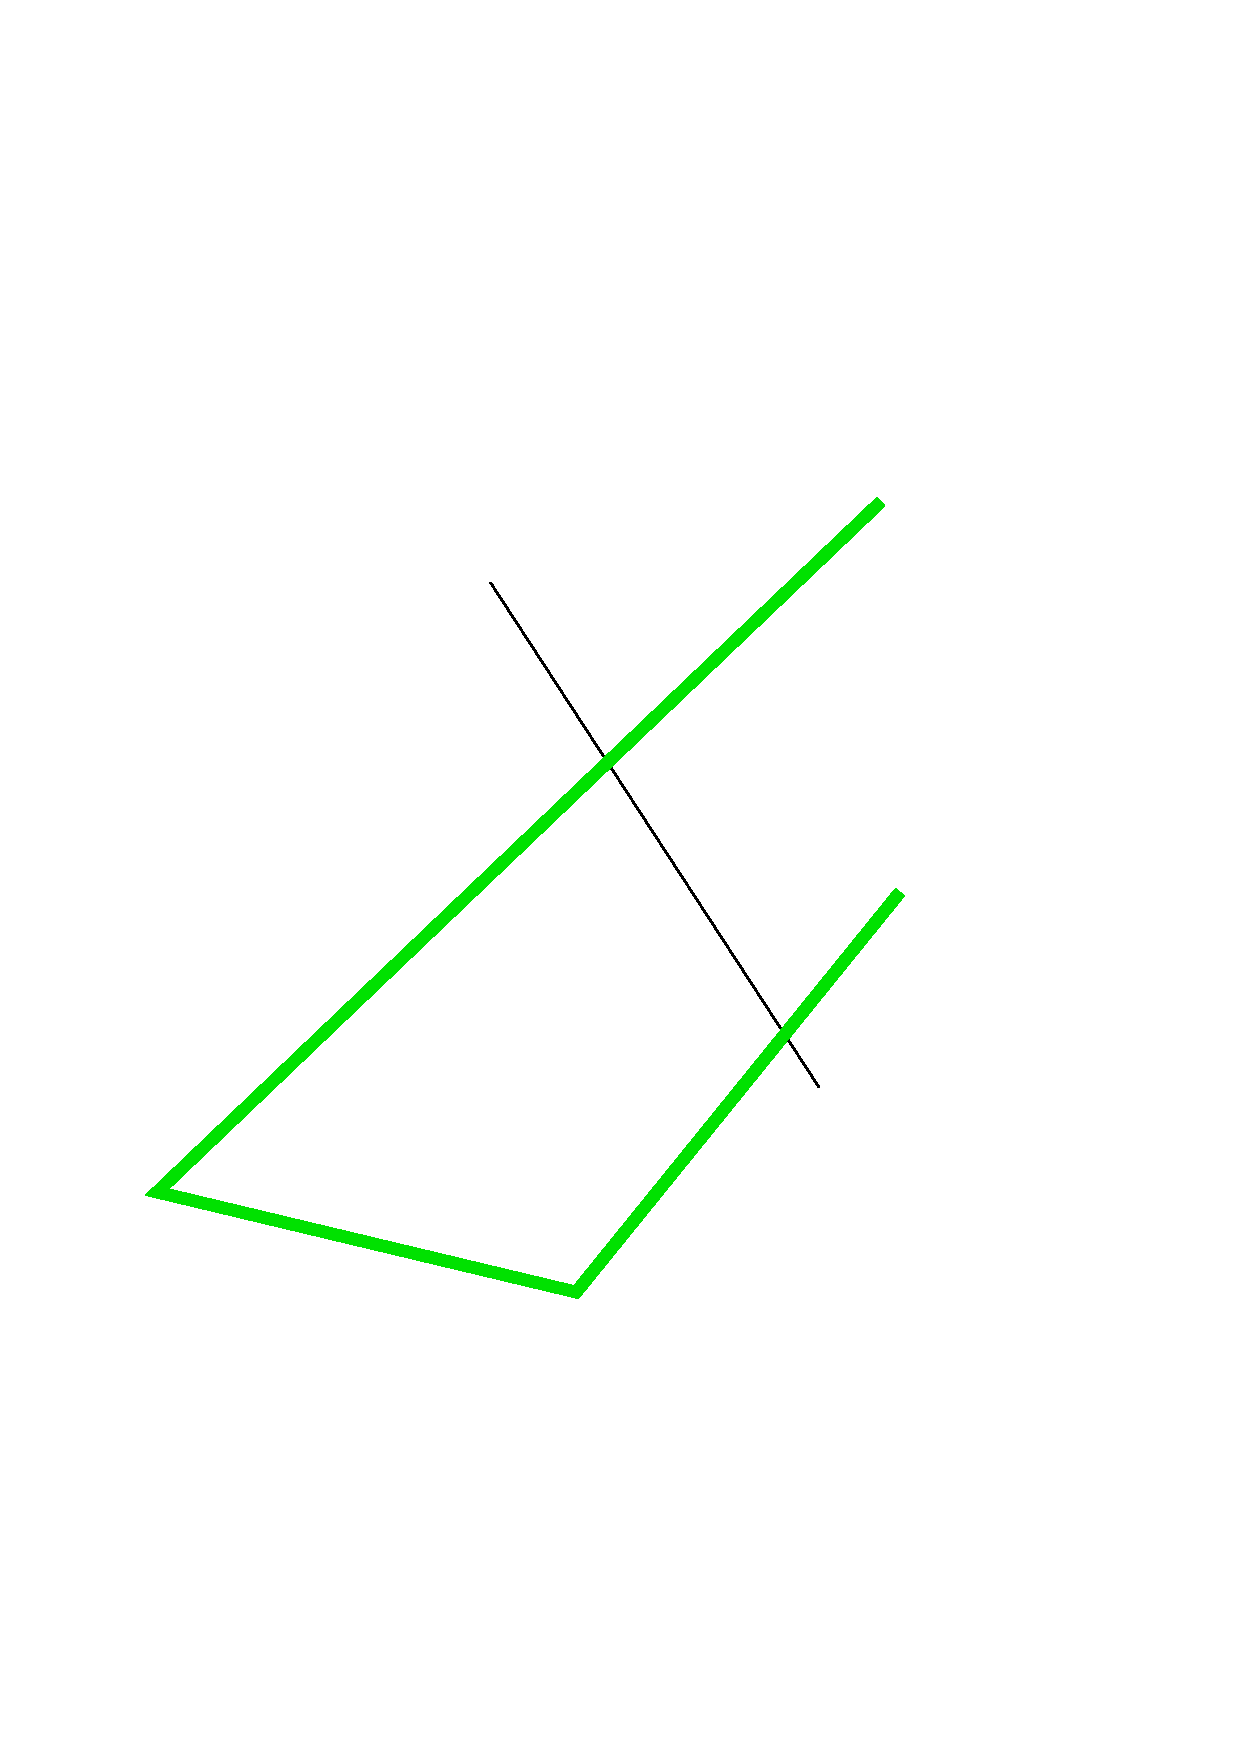
\includegraphics[width=\textwidth]{mydessin.pdf}
  
\includegraphics[bb=0 0 400 300,height=3cm]{test.jpg}
  \caption{La photo originale}
  \label{Photo originale}
\end{figure}

% debut d'une seconde figure
\begin{figure}[h]
    \centering
    \begin{subfigure}[b]{0.3\textwidth}
        
\includegraphics[viewport=0 0 400 300,bb=0 0 400 300,width=4cm,height=3cm,clip=true]{test.jpg}
        \caption{viewport=0 0 400 300\\bb=0 0 400 300}
        \label{essai_a}
    \end{subfigure}
    ~ %add desired spacing between images, e. g. ~, \quad, \qquad etc.
      %(or a blank line to force the subfigure onto a new line)
    \begin{subfigure}[b]{0.3\textwidth}
        
\includegraphics[viewport=160 120 360 270,bb=0 0 400 300,width=4cm,height=3cm,clip=true]{test.jpg}
        \caption{viewport=160 120 360 270\\bb=0 0 400 300}%+200+150
        \label{essai_b}
    \end{subfigure}
    ~
    \begin{subfigure}[b]{0.3\textwidth}
        
\includegraphics[viewport=160 120 320 240,bb=0 0 400 300,width=4cm,height=3cm,clip=true]{test.jpg}
        \caption{viewport=160 120 320 240\\bb=0 0 400 300}%+160+120
        \label{essai_c}
    \end{subfigure}
    \\
    \begin{subfigure}[b]{0.3\textwidth}
        
\includegraphics[viewport=160 120 280 210,bb=0 0 400 300,width=4cm,height=3cm,clip=true]{test.jpg}
        \caption{viewport=160 120 280 210\\bb=0 0 400 300}%+120+90
        \label{essai_d}
    \end{subfigure}
    ~
    \begin{subfigure}[b]{0.3\textwidth}
        
\includegraphics[viewport=160 120 240 180,bb=0 0 400 300,width=4cm,height=3cm,clip=true]{test.jpg}
        \caption{viewport=160 120 240 180\\bb=0 0 400 300}%+80+60
        \label{essai_e}
    \end{subfigure}
    ~
    \begin{subfigure}[b]{0.3\textwidth}
        
\includegraphics[viewport=160 120 200 150,bb=0 0 400 300,width=4cm,height=3cm,clip=true]{test.jpg}
        \caption{viewport=160 120 200 150\\bb=0 0 400 300}%+40+30
        \label{essai_f}
    \end{subfigure}
    \\
    \begin{subfigure}[b]{0.3\textwidth}
        
\includegraphics[viewport=160 120 240 210,bb=0 0 400 300,width=4cm,height=3cm,clip=true]{test.jpg}
        \caption{viewport=160 120 240 210\\bb=0 0 400 300}%+80+90
        \label{essai_g}
    \end{subfigure}
    ~
    \begin{subfigure}[b]{0.3\textwidth}
        
\includegraphics[viewport=160 120 240 180,bb=0 0 400 300,width=4cm,height=3cm,clip=true]{test.jpg}
        \caption{viewport=160 120 240 180\\bb=0 0 400 300}%+80+60
        \label{essai_h}
    \end{subfigure}
    ~
    \begin{subfigure}[b]{0.3\textwidth}
        
\includegraphics[viewport=160 120 240 150,bb=0 0 400 300,width=4cm,height=3cm,clip=true]{test.jpg}
        \caption{viewport=160 120 240 150\\bb=0 0 400 300}%+80+30
        \label{essai_i}
    \end{subfigure}
    \caption{Les options pour l'insertion d'une image :\\viewport variant et bb constant}%\label{fig-double}
    \label{viewport variant et bb constant}

\end{figure}


% debut d'une troisieme figure
\begin{figure}[h]
    \centering
    \begin{subfigure}[b]{0.3\textwidth}
        
\includegraphics[viewport=0 0 400 300,bb=0 0 400 300,width=4cm,height=3cm,clip=true]{test.jpg}
        \caption{viewport=0 0 400 300\\bb=0 0 400 300}
        \label{essai_a}
    \end{subfigure}
    ~
    \begin{subfigure}[b]{0.3\textwidth}
        
\includegraphics[viewport=0 0 400 300,bb=160 120 400 300,width=4cm,height=3cm,clip=true]{test.jpg}
        \caption{viewport=0 0 400 300\\bb=160 120 400 300}
        \label{essai_2}
    \end{subfigure}
    ~
    \begin{subfigure}[b]{0.3\textwidth}
        
\includegraphics[viewport=0 0 400 300,bb=0 0 0 0,width=4cm,height=3cm,clip=true]{test.jpg}
        \caption{viewport=0 0 400 300\\bb=0 0 0 0}
        \label{essai_3}
    \end{subfigure}
    \caption{Les options pour l'insertion d'une image :\\viewport constant et bb inutile}%\label{fig-double}
    \label{viewport constant et bb inutile}

\end{figure}

\subsubsection{trim}
L'option trim fonctionne avec des coordonnées relatives.
Ainsi, {160 120 40 30} correspond à une zone partant du point {160 120}
et allant jusqu'au point situé à {-40 -30} par rapport au point haut droit.
Si l'image de départ a pour dimension {400 300}, alors effectivement, 
en coordonnées absolues, nous avons {160 120 360 270}.
Cela correspond a une image de 200x150.

Sur la figure~\ref{bb constant et trim variant}, page~\pageref{bb constant et trim variant},
nous avons, sur les deux premières lignes, un decoupage sans déformation de l'image, 
tandis que, sur la troisième ligne, nous avons un découpage avec déformation de l'image.

% debut d'une quatrième figure
\begin{figure}[h]
    \centering
    \begin{subfigure}[b]{0.3\textwidth}
        
\includegraphics[bb=0 0 400 300,trim=0 0 0 0,width=4cm,height=3cm,clip=true]{test.jpg}
        \caption{bb=0 0 400 300\\trim=0 0 0 0}
        \label{essai_4}
    \end{subfigure}
    ~
    \begin{subfigure}[b]{0.3\textwidth}
        
\includegraphics[bb=0 0 400 300,trim=160 120 40 30,width=4cm,height=3cm,clip=true]{test.jpg}
        \caption{bb=0 0 400 300\\trim=160 120 40 30}%
        \label{essai_5}
    \end{subfigure}
    ~
    \begin{subfigure}[b]{0.3\textwidth}
        
\includegraphics[bb=0 0 400 300,trim=160 120 80 60,width=4cm,height=3cm,clip=true]{test.jpg}
        \caption{bb=0 0 400 300\\trim=160 120 80 60}%
        \label{essai_6}
    \end{subfigure}
    \\
    \begin{subfigure}[b]{0.3\textwidth}
        
\includegraphics[bb=0 0 400 300,trim=160 120 120 90,width=4cm,height=3cm,clip=true]{test.jpg}
        \caption{bb=0 0 400 300\\trim=160 120 120 90}%
        %
\includegraphics[viewport=0 0 400 300,bb=0 0 400 300,trim=0 0 0 0,width=4cm,height=3cm,clip=true]{test.jpg}
        %\caption{viewport=0 0 400 300\\bb=0 0 400 300\\trim=0 0 0 0}
        \label{essai_4}
    \end{subfigure}
    ~
    \begin{subfigure}[b]{0.3\textwidth}
        
\includegraphics[bb=0 0 400 300,trim=160 120 160 120,width=4cm,height=3cm,clip=true]{test.jpg}
        \caption{bb=0 0 400 300\\trim=160 120 160 120}%
        %
\includegraphics[viewport=0 0 400 300,bb=0 0 400 300,trim=50 50 60 60,width=4cm,height=3cm,clip=true]{test.jpg}
        %\caption{viewport=0 0 400 300\\bb=0 0 400 300\\trim=50 50 60 60}
        \label{essai_5}
    \end{subfigure}
    ~
    \begin{subfigure}[b]{0.3\textwidth}
        \includegraphics[bb=0 0 400 300,trim=160 120 200 150,width=4cm,height=3cm,clip=true]{test.jpg}
        \caption{bb=0 0 400 300\\trim=160 120 200 150}%
        %\includegraphics[viewport=0 0 400 300,bb=0 0 400 300,trim=100 100 110 110,width=4cm,height=3cm,clip=true]{test.jpg}
        %\caption{viewport=0 0 400 300\\bb=0 0 400 300\\trim=100 100 110 110}
        \label{essai_6}
    \end{subfigure}
    \\
    \begin{subfigure}[b]{0.3\textwidth}
        \includegraphics[bb=0 0 400 300,trim=160 120 160 90,width=4cm,height=3cm,clip=true]{test.jpg}
        \caption{bb=0 0 400 300\\trim=160 120 160 90}%deformation
        %\includegraphics[viewport=0 0 400 300,bb=0 0 400 300,trim=0 0 0 0,width=4cm,height=3cm,clip=true]{test.jpg}
        %\caption{viewport=0 0 400 300\\bb=0 0 400 300\\trim=0 0 0 0}
        \label{essai_7}
    \end{subfigure}
    ~
    \begin{subfigure}[b]{0.3\textwidth}
        \includegraphics[bb=0 0 400 300,trim=160 120 160 120,width=4cm,height=3cm,clip=true]{test.jpg}
        \caption{bb=0 0 400 300\\trim=160 120 160 120}
        %\includegraphics[viewport=0 0 400 300,bb=0 0 400 300,trim=50 50 60 60,width=4cm,height=3cm,clip=true]{test.jpg}
        %\caption{viewport=0 0 400 300\\bb=0 0 400 300\\trim=50 50 60 60}
        \label{essai_8}
    \end{subfigure}
    ~
    \begin{subfigure}[b]{0.3\textwidth}
        \includegraphics[bb=0 0 400 300,trim=160 120 160 150,width=4cm,height=3cm,clip=true]{test.jpg}
        \caption{bb=0 0 400 300\\trim=160 120 160 150}
        %\includegraphics[viewport=0 0 400 300,bb=0 0 400 300,trim=100 100 110 110,width=4cm,height=3cm,clip=true]{test.jpg}
        %\caption{viewport=0 0 400 300\\bb=0 0 400 300\\trim=100 100 110 110}
        \label{essai_9}
    \end{subfigure}
    \caption{Les options pour l'insertion d'une image :\\bb constant et trim variant}%\label{fig-double}
    \label{bb constant et trim variant}

\end{figure}


% debut d'une cinquieme figure
\begin{figure}[h]
    \centering
    \begin{subfigure}[b]{0.3\textwidth}
        \includegraphics[bb=0 0 400 300,trim=0 0 0 0,width=4cm,height=3cm,clip=true]{test.jpg}
        \caption{bb=0 0 400 300\\trim=0 0 0 0}
        \label{essai_a}
    \end{subfigure}
    ~
    \begin{subfigure}[b]{0.3\textwidth}
        \includegraphics[bb=160 120 560 420,trim=0 0 0 0,width=4cm,height=3cm,clip=true]{test.jpg}
        \caption{bb=160 120 560 420\\trim=0 0 0 0}
        \label{essai_2}
    \end{subfigure}
    ~
    \begin{subfigure}[b]{0.3\textwidth}
        \includegraphics[bb=160 120 400 300,trim=0 0 0 0,width=4cm,height=3cm,clip=true]{test.jpg}
        \caption{bb=160 120 400 300\\trim=0 0 0 0}
        \label{essai_3}
    \end{subfigure}
    \caption{Les options pour l'insertion d'une image :\\bb inutile et trim constant}%\label{fig-double}
    \label{bb inutile et trim constant}

\end{figure}


% debut d'une troisieme figure
\begin{figure}[!h]
\centering
%\includegraphics[width=\textwidth]{mydessin.pdf}
\includegraphics[width=300pt]{mydessin.pdf}
\caption{Ceci est encore mydessin.pdf}
\label{mydessin3}
\end{figure}

% debut d'une quatrieme figure
\begin{figure}[!h]
\centering
%\includegraphics[width=\textwidth]{mydessin.pdf}
\includegraphics[width=400pt]{mydessin.pdf}
\caption{Ceci est encore et toujours mydessin.pdf}
\label{mydessin4}
\end{figure}

% reference a une figure
Sur la figure~\ref{mydessin1}, page~\pageref{mydessin1}, nous avons mis une largeur de 100 pt.

Sur la figure~\ref{mydessin2}, page~\pageref{mydessin2}, nous avons mis une largeur de 200 pt.

Sur la figure~\ref{mydessin3}, page~\pageref{mydessin3}, nous avons mis une largeur de 300 pt.

Sur la figure~\ref{mydessin4}, page~\pageref{mydessin4}, nous avons mis une largeur de 400 pt.

% liste des figures
\listoffigures

\end{document}



% liste des figures
\listoffigures

\end{document}
